%%%%%%%% NATURE COMPUTATIONAL SCIENCE LATEX MANUSCRIPT %%%%%%%%%%%%%%%%
%
% Deterministic conversion of paper/paper2/paper2-ncs-en.md
% Style: Nature Portfolio / Nature Computational Science (sn-ncs.sty)
%%%%%%%%%%%%%%%%%%%%%%%%%%%%%%%%%%%%%%%%%%%%%%%%%%%%%%%%%%%%%%%%%%%%%%%

\documentclass[10pt,a4paper]{article}

\usepackage{sn-ncs}

\ncstitle{Training-free mean-field adjoint manifold initialization for constrained variational quantum optimization}
\ncsauthor{Jianxuan Yao}
\ncsaffiliation{ShanghaiTech University, Shanghai, China}
\ncsemail{yaojx2025@shanghaitech.edu.cn}

\begin{document}

\makencstitle


\begin{ncsabstract}

Constrained combinatorial optimization with the Quantum Approximate Optimization Algorithm (QAOA) must navigate rugged landscapes induced by competing local fields and quadratic spin couplings. Homogeneous annealing ramps apply uniform phases across qubits and require dozens of noisy online measurements for selection, whereas warm-start schemes alter the circuit ansatz and forfeit native global-pulse execution. Here we prove that within the unmodified depth-$2k$ global QAOA circuit, anti-symmetric cost pairing with odd-layer spin flips achieves $2k$-dimensional parity cancellation of quadratic couplings, establishing an exact quantum-classical product-energy identity. Exploiting this identity, we introduce \texttt{Echo-MF-2kD}, a training-free initializer integrating temperature-continuation mean-field orientation, Daubechies maximally flat anchors, and $O(kn)$ $\mathrm{SU}(2)$-adjoint refinement. Across 1,024 Maximum Weight Independent Set instances at $n=10$ and 5,120 cross-scale instances spanning $n=6\mbox{--}14$, \texttt{Echo-MF-2kD} requires zero Stage-1 measurements, doubles Trotterized Quantum Annealing ground-state probability ($46.16\%$ versus $22.42\%$ at $n=10$), cuts Stage-2 quantum calls by $45.2\%$, and achieves $100\%$ shot-noise selection immunity.

\end{ncsabstract}

\section*{Introduction}

Constrained combinatorial optimization problems---such as Maximum Weight Independent Set (MWIS)---arise across network allocation and statistical physics, mapping to Ising Hamiltonians $H_C = H_J + H_h + C$ over $n$ spins $s \in \{-1, +1\}^n$ \citep{lucas2014ising,pichler2018quantum,ebadi2022quantum}. Under hard-constraint penalties, heterogeneous vertex degrees induce strong site-specific local fields $H_h = \sum_i h_i S_i$ competing with repulsive quadratic couplings $H_J = \sum_{i<j} J_{ij} S_i S_j$ \citep{hadfield2019quantum}. The Quantum Approximate Optimization Algorithm (QAOA) prepares a $p$-layer state $|\psi_p(\vartheta)\rangle = \prod_{\ell=1}^p U_B(\beta_\ell) U_C(\gamma_\ell) |+\rangle^{\otimes n}$ via cost unitaries $U_C(\gamma_\ell) = e^{-i\gamma_\ell H_C}$ and global transverse-field mixers $U_B(\beta_\ell) = e^{-i\beta_\ell \sum_i X_i}$ \citep{farhi2014quantum,preskill2018quantum,cerezo2021variational,blekos2024review}. Preserving $|+\rangle^{\otimes n}$ and global mixers $U_B(\beta_\ell)$ is vital for superconducting processors \citep{harrigan2021quantum}, trapped-ion simulators \citep{pagano2020quantum}, and Rydberg atom arrays \citep{ebadi2022quantum}, where a single global pulse drives all qubits natively. At fixed depth $p$, however, the non-convex $2p$-dimensional energy landscape contains exponentially many suboptimal minima and symmetric branches \citep{mcclean2018barren,shaydulin2019multistart,lotshaw2021empirical,shaydulin2021classical,you2021exponentially,bittel2021training,anschuetz2022quantum}. Because each parameter-shift gradient step requires $O(p)$ circuit executions and thousands of measurement shots \citep{mitarai2018quantum,wierichs2022general}, computing a high-overlap starting point $\vartheta_0 \in \mathbb{R}^{2p}$ solely from $(J, h)$ without circuit modification or online selection measurements is a central challenge.

Existing QAOA initializers face fundamental trade-offs under heterogeneous local fields. First, homogeneous schedules---including Trotterized Quantum Annealing (TQA) \citep{farhi2001quantum,kadowaki1998quantum,yang2017optimizing,sack2021quantum,wurtz2022counterdiabaticity}, layerwise interpolation (INTERP) \citep{crooks2018performance,zhou2020quantum}, and parameter transfer \citep{brandao2018fixed,galda2021transferability,shaydulin2023parameter}---apply identical phase ramps across all qubits and cannot resolve site-specific spin orientations on conflicting edges \citep{katial2025instance}; moreover, online TQA requires dozens of Stage-1 quantum evaluations vulnerable to shot-noise misselection ("Winner's Curse"). Second, ansatz-modifying schemes such as Semidefinite-Programming (SDP) Warm-Start QAOA \citep{bravyi2020obstacles,egger2021warm,tate2023warm} and multi-angle \texttt{ma-QAOA} \citep{herrman2022multi} either replace uniform mixers with custom rotations that forfeit global-pulse compatibility and induce spin-freezing dead zones, or inflate parameter dimension to $O(p(|V|+|E|))$ at prohibitive measurement cost. Third, spin-echo parity decoupling within the standard global circuit \citep{hahn1950spin,carr1954effects,viola1999dynamical,vandersypen2005nmr,yao2026echo} pairs anti-symmetric cost angles $(-g_j, g_j)$ with odd-layer flips $\beta_{2j-1} = \pi/2$ to cancel $H_J$ along a one-dimensional (1D) scalar ray $g_j = a r_j$ \citep{daubechies1988orthonormal,low2016methodology,low2017optimal,gilyen2019quantum,yao2026echo}. Without offline supervision, however, restricting all $k$ pairs to one scalar $a$ encounters two barriers when $n > 2k$: (1) \emph{Diophantine frequency crowding}, where one scalar cannot align $n > 2k$ incommensurate frequencies $4h_i$; and (2) \emph{local effective-field inversion}, where weakly polarized qubits suffer repulsive pulls $(J\boldsymbol{m})_i$ upon Stage-2 coupling reactivation, flipping their local effective field $h_i^{\mathrm{eff}}(\boldsymbol{m}) = h_i + (J\boldsymbol{m})_i$.

To overcome both barriers without circuit modification or quantum measurements, we observe that parity cancellation of $H_J$ is an intra-pair algebraic identity rather than a 1D property. Because each spin-echo pair conjugates $H_C$ by the global flip operator $F = \prod_{i=1}^n X_i$ independently, exact cancellation of $H_J$ holds across the entire $2k$-dimensional complete-pair submanifold where all $k$ cost half-angles $\boldsymbol{g} \in \mathbb{R}^k$ and $k$ even-layer mixer angles $\boldsymbol{\theta} \in \mathbb{R}^k$ vary freely. On this $2k$-dimensional manifold, the $2p$-layer state factorizes strictly into single-qubit states computable in $O(kn)$ classical $2\times 2$ operations, and inter-qubit independence guarantees that the multi-body quantum expected energy equals the classical product-state energy identically: $\langle\psi_p(\boldsymbol{g},\boldsymbol{\theta})|H_C|\psi_p(\boldsymbol{g},\boldsymbol{\theta})\rangle \equiv E_{\mathrm{prod}}(\boldsymbol{g},\boldsymbol{\theta})$. This identity reduces quantum initialization to a differentiable classical control problem on $\mathrm{SU}(2)^{\otimes n}$ that anticipates multi-body coupling effects via $E_{\mathrm{prod}}$ and $h_i^{\mathrm{eff}}(\boldsymbol{m})$ before any quantum circuit runs.

Here we introduce Mean-Field Multi-Scalar Adjoint Product-Manifold Initialization (\texttt{Echo-MF-2kD}), a training-free, zero-quantum-selection framework mapping $(J, h)$ directly to standard $2p$-dimensional global QAOA angles. For non-vanishing local fields ($h_i \ne 0$) at positive even depth $p = 2k$, we prove that the $2k$-dimensional complete-pair submanifold preserves exact product factorization and product-energy equivalence while guaranteeing first-order linear reactivation of $H_J$ under symmetry-breaking Stage-2 perturbations. Algorithmically, \texttt{Echo-MF-2kD} resolves edge repulsion into a self-consistent binary orientation $\hat{\boldsymbol{s}} \in \{-1, +1\}^n$ via damped mean-field temperature continuation and single-edge cluster flips, extracts resonance anchors using the strict convexity of 1D Daubechies responses on zero-free intervals, and performs staged $O(kn)$ reverse-mode $\mathrm{SU}(2)$-adjoint refinement within a non-degenerate mixer domain to optimize flip-sensitivity-weighted log-likelihood, local effective-field inversion guards, and $E_{\mathrm{prod}}$, followed by Stage-2 full-angle recoupling \citep{dupont2022entanglement}. Across 1,024 held-out MWIS instances at $n=10$, 5,120 cross-scale instances ($n \in \{6, 8, 10, 12, 14\}$), and 2,750 five-family benchmark instances, \texttt{Echo-MF-2kD} doubles online TQA ground-state probability at $n=10$ ($46.16\%$ versus $22.42\%$, reaching $60.80\%$ at $p=12$) with zero Stage-1 measurements, $45.2\%$ fewer Stage-2 quantum calls, and $100\%$ Stage-1 shot-noise immunity.


\section*{Results}

\subsection*{Exact product-energy identity on the \texorpdfstring{$2k$}{2k}-dimensional spin-echo manifold}

\begin{figure}[!htbp]
\centering
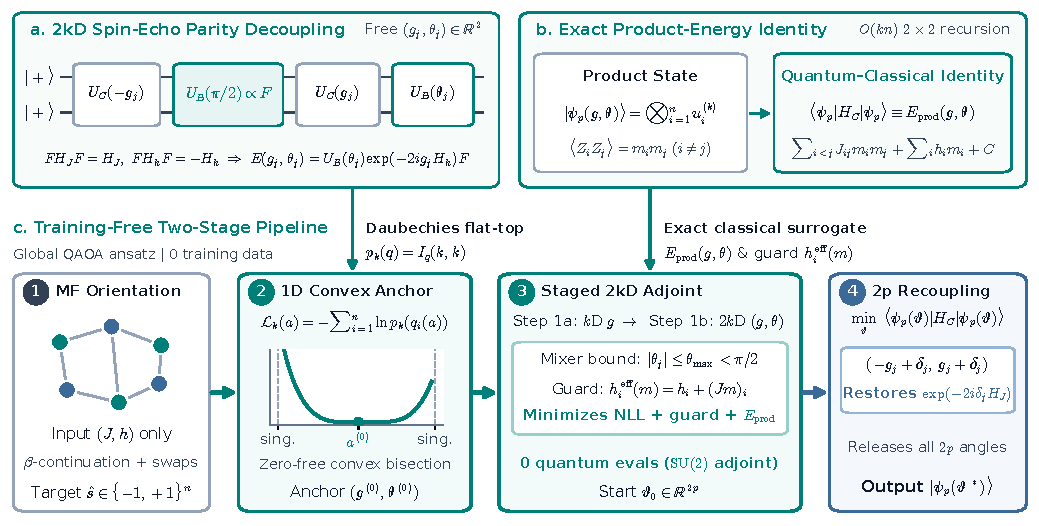
\includegraphics[width=0.96\textwidth]{figures/fig1_echo_mf_2kd_overview.pdf}
\vspace{-2pt}
\caption{\textbf{Algorithmic architecture and physical mechanism of \texttt{Echo-MF-2kD}.} Given an unseen problem instance $(J, h)$, Stage 1 operates entirely on a classical processor with zero online quantum evaluations: damped mean-field temperature continuation and single-edge cluster flips first lock onto a self-consistent binary target orientation $\hat{\boldsymbol{s}} \in \{-1, +1\}^n$; 1D Daubechies maximally flat convex-interval root extraction then identifies resonance anchors $(\boldsymbol{g}^{(0)}, \boldsymbol{\theta}^{(0)})$; finally, staged $O(kn)$ reverse-mode $\mathrm{SU}(2)$-adjoint optimization refines all $2k$ intra-pair parameters on the complete spin-echo product manifold under non-degenerate mixer bounds, local effective-field inversion guards, and the exact classical product energy $E_{\mathrm{prod}}$ to produce standard $2p$-dimensional global QAOA angles $\vartheta_0$. Stage 2 releases all $2p$ angles in a standard L-BFGS-B quantum energy optimizer, breaking pair anti-symmetry to activate multi-body entanglement and converge rapidly to the true ground state $s^\star$.}
\label{fig:1}
\end{figure}

In a standard global QAOA circuit of positive even depth $p = 2k$, pairing adjacent layers $2j-1$ and $2j$ ($j = 1, \ldots, k$) with anti-symmetric cost angles $(\gamma_{2j-1}, \gamma_{2j}) = (-g_j, g_j)$ and mixer angles $(\beta_{2j-1}, \beta_{2j}) = (\pi/2, \theta_j)$ sets every odd-layer mixer equal to the global spin-flip operator $U_B(\pi/2) = (-i)^n F$, where $F = \prod_{i=1}^n X_i$. Because quadratic spin-spin couplings are even under global spin inversion ($F H_J F = H_J$) whereas local external fields are odd ($F H_h F = -H_h$), the composite unitary of the $j$-th pair simplifies identically to $E(g_j, \theta_j) = U_B(\theta_j) e^{-2i g_j H_h} F$ up to a global phase \citep{yao2026echo} (Methods). Crucially, this operator cancellation occurs \emph{within each pair individually} and imposes no cross-pair ratio constraints on $(g_j, \theta_j)$. Consequently, across the entire $2k$-dimensional complete-pair parameter submanifold $(\boldsymbol{g}, \boldsymbol{\theta}) = (g_1, \ldots, g_k, \theta_1, \ldots, \theta_k) \in [-10\pi, 10\pi]^k \times [-\pi/2, \pi/2)^k$, the $2p$-layer quantum circuit output factorizes strictly into a tensor product of single-qubit states $|\psi_p(\boldsymbol{g}, \boldsymbol{\theta})\rangle = \bigotimes_{i=1}^n u_i^{(k)}(\boldsymbol{g}, \boldsymbol{\theta})$, whose positive-spin probabilities $p_i^+(\boldsymbol{g}, \boldsymbol{\theta}) = |u_{i,+}^{(k)}|^2$ and magnetizations $m_i(\boldsymbol{g}, \boldsymbol{\theta}) = 2p_i^+ - 1 \in [-1, 1]$ are evaluated deterministically in $O(kn)$ time via $k$ steps of $2\times 2$ unitary recursion. Because Pauli-$Z$ observables on distinct qubits are statistically independent in any product state ($\langle Z_i Z_j \rangle = m_i m_j$ for $i \ne j$), the multi-body quantum expected energy on the $2k$-dimensional submanifold equals the classical product-state energy identically:
\[
\langle\psi_p(\boldsymbol{g},\boldsymbol{\theta})|H_C|\psi_p(\boldsymbol{g},\boldsymbol{\theta})\rangle \equiv E_{\mathrm{prod}}(\boldsymbol{g},\boldsymbol{\theta}) = \frac{1}{2}\boldsymbol{m}(\boldsymbol{g},\boldsymbol{\theta})^\top J\boldsymbol{m}(\boldsymbol{g},\boldsymbol{\theta}) + \boldsymbol{h}^\top\boldsymbol{m}(\boldsymbol{g},\boldsymbol{\theta}) + C.
\]
Furthermore, perturbing the $j$-th pair's cost angles along the symmetry-breaking coordinate $(-g_j + \delta_j, g_j + \delta_j)$ in Stage 2 yields the pair operator $U_B(\theta_j) e^{-2i\delta_j H_J} e^{-2i g_j H_h} F$, which re-activates quadratic coupling evolution $H_J$ linearly to first order in $\delta_j$ and guarantees non-vanishing tangent gradients upon departing the product manifold (Methods).

This exact quantum--classical correspondence enables classical optimization of $E_{\mathrm{prod}}(\boldsymbol{g}, \boldsymbol{\theta})$ and single-qubit phase alignment across all $2k$ degrees of freedom with zero quantum circuit executions (Figure 1). Our framework (\texttt{Echo-MF-2kD} in online training-free mode; \texttt{Echo-Flat-2kD} in offline known-target analysis) comprises three mechanistic stages detailed in Methods: (1) \emph{deterministic temperature-continuation cluster orientation}, which continues damped mean-field magnetizations across an ascending inverse-temperature schedule with zero-temperature single-edge cluster swaps to resolve soft-marginal ambiguity into a self-consistent binary orientation $\hat{\boldsymbol{s}} \in \{-1, +1\}^n$; (2) \emph{Daubechies maximally flat convex-interval anchor extraction}, which exploits the strict convexity of 1D Daubechies negative log-likelihood on zero-free intervals to extract resonance anchors $(\boldsymbol{g}^{(0)}, \boldsymbol{\theta}^{(0)})$ via bisection; and (3) \emph{staged $O(kn)$ reverse-mode $\mathrm{SU}(2)$-adjoint refinement}, which backpropagates analytical gradients through the $k$-step $2\times 2$ spinor recursion (Step 1a aligning $k$ cost angles $\boldsymbol{g}$, Step 1b jointly refining $(\boldsymbol{g}, \boldsymbol{\theta})$ within a non-degenerate mixer bound $|\theta_j| \le \theta_{\max} < \pi/2$) to optimize flip-sensitivity-weighted log-likelihood, local effective-field inversion guards, and $E_{\mathrm{prod}}$.

\begin{table}[!htbp]
\caption{\textbf{Progressive component ablation from 1D scalar scanning to guarded staged $2k$D manifold refinement on unseen MWIS test sets.} Values report mean initial $\rightarrow$ post-optimization ground-state probabilities $P_{\mathrm{gs}}^{\mathrm{init}} \rightarrow P_{\mathrm{gs}}^{\mathrm{final}}$ (\%) with 4,000-resample bootstrap 95\% confidence intervals (CIs) and Stage-1 all-qubit quadrant hit rates ($\forall i: h_i \ne 0, \pi_i > 0.50$, in parentheses) across $n \in \{8, 10, 12\}$ at fixed depth $p = 10$ ($k = 5$ pairs; 1,024 unseen test instances per scale). Both offline known-target mode (\texttt{Echo-Flat-{*}}) and online training-free mode (\texttt{Echo-MF-{*}}, taking only $(J, h)$ with zero online quantum selection evaluations) are evaluated under identical Stage-2 L-BFGS-B settings. Bold values denote the best final ground-state probability within each mode.}
\label{tab:1}
\vspace{2pt}
\centering
\renewcommand{\arraystretch}{1.15}
\setlength{\tabcolsep}{3.5pt}
\resizebox{\textwidth}{!}{%
\begin{tabular}{llccc}
\toprule
\shortstack[l]{\textbf{Mode \&} \\ \textbf{Ablation Variant}} & \shortstack[l]{\textbf{Active Degrees of Freedom} \\ \textbf{\& Adjoint Physical Guards}} & \shortstack[c]{\textbf{$n = 8$} \\ \textbf{($P_{\mathrm{gs}}^{\mathrm{init}} \rightarrow P_{\mathrm{gs}}^{\mathrm{final}}$, Quad. Hit)}} & \shortstack[c]{\textbf{$n = 10$} \\ \textbf{($P_{\mathrm{gs}}^{\mathrm{init}} \rightarrow P_{\mathrm{gs}}^{\mathrm{final}}$, Quad. Hit)}} & \shortstack[c]{\textbf{$n = 12$} \\ \textbf{($P_{\mathrm{gs}}^{\mathrm{init}} \rightarrow P_{\mathrm{gs}}^{\mathrm{final}}$, Quad. Hit)}} \\
\midrule
\textbf{Offline \texttt{Echo-Flat-1D}} & $1$-D scalar $a$, Flat-Top convex-interval bisection & $33.19 \rightarrow 77.25^{+1.36}_{-1.34}\%$ ($46.0\%$) & $13.07 \rightarrow 53.08^{+1.51}_{-1.57}\%$ ($18.8\%$) & $3.69 \rightarrow 29.64^{+1.33}_{-1.25}\%$ ($4.4\%$) \\
\textbf{Offline \texttt{Echo-Flat-kD (Cost-Only)}} & $k$-D cost $\boldsymbol{g}$, fixed $\boldsymbol{\theta}^{(0)}$, unweighted unguarded NLL & $35.02 \rightarrow 78.47^{+1.19}_{-1.23}\%$ ($69.0\%$) & $15.17 \rightarrow 55.73^{+1.37}_{-1.38}\%$ ($37.7\%$) & $4.91 \rightarrow 33.63^{+1.22}_{-1.14}\%$ ($17.3\%$) \\
\textbf{Offline \texttt{Echo-Flat-kD (Guarded)}} & $k$-D cost $\boldsymbol{g}$, weighted inversion guard + $\alpha_E E_{\mathrm{prod}}$ & $33.05 \rightarrow 78.35^{+1.21}_{-1.24}\%$ ($49.3\%$) & $13.66 \rightarrow 54.79^{+1.47}_{-1.49}\%$ ($22.7\%$) & $4.09 \rightarrow 32.50^{+1.19}_{-1.22}\%$ ($6.5\%$) \\
\textbf{Offline \texttt{Echo-Flat-2kD (Unconstrained)}} & $2k$-D full pair $(\boldsymbol{g},\boldsymbol{\theta})$, unguarded unstaged & $71.52 \rightarrow 84.53^{+0.94}_{-0.95}\%$ ($94.4\%$) & $45.45 \rightarrow 64.03^{+1.20}_{-1.25}\%$ ($88.8\%$) & $23.40 \rightarrow 41.36^{+1.19}_{-1.19}\%$ ($77.8\%$) \\
\textbf{Offline \texttt{Echo-Flat-2kD}} & $2k$-D staged refinement, non-degenerate mixer + inversion guard + $E_{\mathrm{prod}}$ & $70.89 \rightarrow \mathbf{85.01}^{+0.92}_{-0.93}\%$ ($94.0\%$) & $44.31 \rightarrow \mathbf{64.29}^{+1.22}_{-1.24}\%$ ($86.4\%$) & $22.87 \rightarrow \mathbf{41.41}^{+1.18}_{-1.15}\%$ ($75.0\%$) \\
\textbf{Online Training-Free \texttt{Echo-MF-Flat} (\texttt{Echo-MF-1D})} & Mean-field soft marginals + $1$-D overlap decoding & $15.96 \rightarrow 45.11^{+2.41}_{-2.40}\%$ ($0.0\%$) & $5.39 \rightarrow 23.23^{+1.83}_{-1.92}\%$ ($0.0\%$) & $1.26 \rightarrow 9.74^{+1.21}_{-1.12}\%$ ($0.0\%$) \\
\textbf{Online Training-Free \texttt{Echo-MF-kD (Soft,\allowbreak\ Cost-Only)}} & Mean-field soft marginals + unguarded $k$-D cost refinement & $21.08 \rightarrow 46.96^{+2.36}_{-2.35}\%$ ($73.2\%$) & $8.16 \rightarrow 23.83^{+1.82}_{-1.77}\%$ ($39.6\%$) & $2.51 \rightarrow 9.65^{+1.08}_{-1.04}\%$ ($22.0\%$) \\
\textbf{Online Training-Free \texttt{Echo-MF-kD (Guarded)}} & Temp.-continuation cluster orientation + guarded $k$-D cost & $32.47 \rightarrow 61.64^{+2.17}_{-2.26}\%$ ($49.2\%$) & $13.03 \rightarrow 31.58^{+1.99}_{-1.96}\%$ ($22.5\%$) & $3.89 \rightarrow 12.31^{+1.27}_{-1.26}\%$ ($6.3\%$) \\
\textbf{Online Training-Free \texttt{Echo-MF-2kD (Unconstrained)}} & Temp.-continuation cluster orientation + unguarded $2k$-D & $70.03 \rightarrow 74.69^{+1.64}_{-1.69}\%$ ($94.3\%$) & $43.20 \rightarrow \mathbf{46.75}^{+1.77}_{-1.85}\%$ ($88.8\%$) & $21.88 \rightarrow 22.39^{+1.30}_{-1.35}\%$ ($77.9\%$) \\
\textbf{Online Training-Free \texttt{Echo-MF-2kD}} & Temp.-continuation cluster orientation + guarded staged $2k$-D & $69.41 \rightarrow \mathbf{74.99}^{+1.65}_{-1.68}\%$ ($93.8\%$) & $42.20 \rightarrow 46.70^{+1.78}_{-1.90}\%$ ($86.8\%$) & $21.38 \rightarrow \mathbf{22.64}^{+1.31}_{-1.38}\%$ ($75.0\%$) \\
\bottomrule
\end{tabular}%
}
\end{table}
Controlled ablations across 5,120 unseen MWIS instances confirm the distinct physical role of each mechanism (Table 1). First, in online unsupervised mode, fitting unoriented soft mean-field marginals (\texttt{Echo-MF-kD (Soft,\allowbreak\ Cost-Only)}) stalls at $23.83\%$ ($n=10$) and $9.65\%$ ($n=12$) because frustrated vertices with $\pi_i^{\mathrm{mf}} \approx 0.5$ pull optimization toward incompatible independent-set branches. Introducing deterministic temperature-continuation cluster orientation and effective-field inversion guards (\texttt{Echo-MF-kD (Guarded)}) lifts single-qubit spin orientation accuracy from $85.03\%\mbox{--}89.18\%$ to $93.75\%\mbox{--}99.61\%$ and raises online final probabilities by $+14.68$ and $+7.75$ percentage points (pp) at $n=8, 10$. Second, when system size exceeds the pair count ($n \ge 10 > k = 5$), tuning only the $k=5$ cost angles with frozen 1D Daubechies mixers (\texttt{Echo-Flat-kD} and \texttt{Echo-MF-kD}) cannot resolve Diophantine frequency crowding, limiting $n=12$ initial product probabilities to $3.89\%\mbox{--}4.91\%$ and all-qubit quadrant hit rates to $6.3\%\mbox{--}17.3\%$. Releasing all $2k=10$ parameters in Step 1b (\texttt{Echo-Flat-2kD} and \texttt{Echo-MF-2kD}) boosts the $n=12$ initial product probability more than fivefold to $21.38\%\mbox{--}22.87\%$ and lifts the quadrant hit rate to $75.0\%$ ($86.4\%\mbox{--}86.8\%$ at $n=10$). Third, enforcing the non-degenerate mixer bound and staged inversion guards yields the highest cross-scale performance (\texttt{Echo-Flat-2kD} reaching $\mathbf{85.01}\%, \mathbf{64.29}\%, \mathbf{41.41}\%$ at $n=8, 10, 12$; online \texttt{Echo-MF-2kD} reaching $\mathbf{94.02}\%, \mathbf{74.99}\%, \mathbf{46.70}\%, \mathbf{22.64}\%, \mathbf{10.13}\%$ across $n=6\mbox{--}14$), outperforming 1D \texttt{Echo-MF-Flat} by $+5.81\mbox{--}{+}29.88$ pp while cutting Stage-2 quantum gradient evaluations from $102.3\mbox{--}122.5$ down to $\mathbf{61.3\mbox{--}79.3}$.


\subsection*{Doubling ground-state probability while halving quantum search cost}

\begin{figure}[!htbp]
\centering
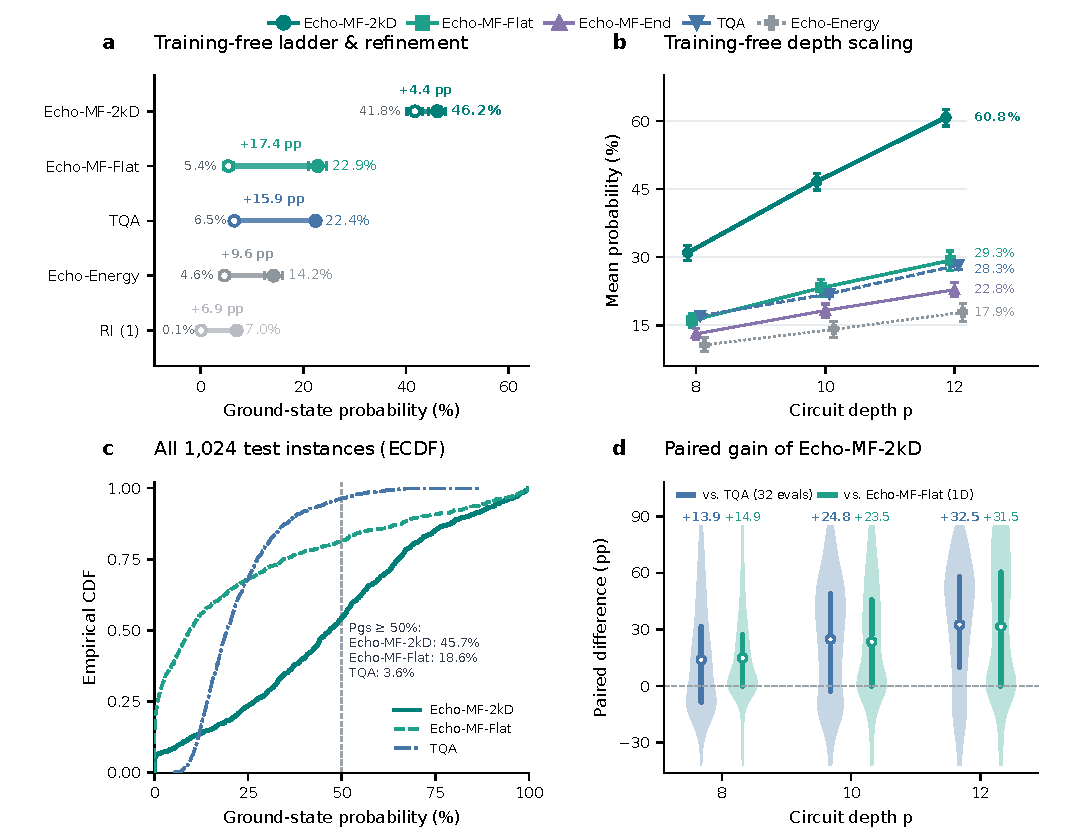
\includegraphics[width=0.92\textwidth]{figures/mf-echo-comparison.pdf}
\vspace{-2pt}
\caption{\textbf{\texttt{Echo-MF-2kD} more than doubles the final ground-state probability of online TQA while halving Stage-2 quantum gradient calls on held-out MWIS instances ($n=10$, 1,024 unseen test instances).} \textbf{a}, Cross-depth instance-averaged Stage-1 initial product-state ground-state probability $P_{\mathrm{gs}}^{(0)}$ and Stage-2 post-optimization final ground-state probability $P_{\mathrm{gs}}$ across $p \in \{8, 10, 12\}$. \textbf{b}, Final mean ground-state probability scaling as a function of circuit depth $p = 8, 10, 12$; error bars denote 4,000-resample non-parametric percentile bootstrap 95\% CIs. \textbf{c}, Empirical cumulative distribution functions (ECDFs) of cross-depth mean final ground-state probability across all 1,024 test instances, highlighting high-probability instance coverage ($P_{\mathrm{gs}} \ge 50\%$). \textbf{d}, Per-instance paired net probability gains ($\Delta P_{\mathrm{gs}}$, in percentage points) of \texttt{Echo-MF-2kD} over 32-evaluation online TQA and 1D \texttt{Echo-MF-Flat} across circuit depths.}
\label{fig:2}
\end{figure}

\begin{table}[!htbp]
\caption{\textbf{Stage-wise quantum evaluation cost and initial-to-final ground-state probabilities on the held-out MWIS center test set ($n=10$, 1,024 unseen instances).} All methods receive only $(J, h)$ with zero training data and execute identical Stage-2 full-angle L-BFGS-B energy optimization. Values report Stage-1 online quantum circuit evaluations, Stage-2 gradient quantum evaluations at $p = 8 / 10 / 12$ (and cross-depth mean), initial $\rightarrow$ final mean ground-state probabilities (\%) with 4,000-resample bootstrap 95\% CIs, and paired net differences relative to 32-evaluation online TQA. Bold indicates the best performance in each column.}
\label{tab:2}
\vspace{2pt}
\centering
\renewcommand{\arraystretch}{1.15}
\setlength{\tabcolsep}{3.5pt}
\resizebox{\textwidth}{!}{%
\begin{tabular}{llccccccc}
\toprule
\textbf{Method Name} & \shortstack[l]{\textbf{Prior Source \& Initialization Mechanism} \\ \textbf{(Input $J,h$ Only, 0 Training Data)}} & \shortstack[c]{\textbf{Stage-1 Online} \\ \textbf{Quantum Evals}} & \shortstack[c]{\textbf{Stage-2 Gradient Quantum} \\ \textbf{Evals ($p=8 / 10 / 12$, Mean)}} & \shortstack[c]{\textbf{$p = 8$} \\ \textbf{($P_{\mathrm{gs}}^{(0)} \rightarrow P_{\mathrm{gs}}$)}} & \shortstack[c]{\textbf{$p = 10$} \\ \textbf{($P_{\mathrm{gs}}^{(0)} \rightarrow P_{\mathrm{gs}}$)}} & \shortstack[c]{\textbf{$p = 12$} \\ \textbf{($P_{\mathrm{gs}}^{(0)} \rightarrow P_{\mathrm{gs}}$)}} & \shortstack[c]{\textbf{Cross-Depth} \\ \textbf{Mean $P_{\mathrm{gs}}^{(0)} \rightarrow P_{\mathrm{gs}}$}} & \shortstack[c]{\textbf{Cross-Depth Paired} \\ \textbf{Gain vs. TQA (pp)}} \\
\midrule
\textbf{RI (1)} & Prior-free, single-start random initialization & $0$ & $110.1 / 130.4 / 135.1$ ($125.2$) & $0.10 \rightarrow 3.84^{+0.60}_{-0.57}$ & $0.10 \rightarrow 6.82^{+0.90}_{-0.87}$ & $0.10 \rightarrow 10.42^{+1.23}_{-1.20}$ & $0.10 \rightarrow 7.03\%$ & $-15.39\ ([-16.18, -14.65])$ \\
\textbf{RI (32)} & Prior-free, 32-candidate random angles with quantum energy selection & $32$ & $123.8 / 136.9 / 141.2$ ($134.0$) & $0.22 \rightarrow 6.47^{+0.62}_{-0.60}$ & $0.20 \rightarrow 9.93^{+0.87}_{-0.81}$ & $0.17 \rightarrow 12.81^{+1.02}_{-0.97}$ & $0.20 \rightarrow 9.73\%$ & $-12.69\ ([-13.41, -11.98])$ \\
\textbf{Echo-Energy} & Prior-free, 1D Flat-Top product-energy selection & $0$ & $58.8 / 94.9 / 125.4$ ($93.0$) & $4.34 \rightarrow 10.68^{+1.54}_{-1.48}$ & $4.70 \rightarrow 14.09^{+1.77}_{-1.75}$ & $4.91 \rightarrow 17.86^{+2.03}_{-1.94}$ & $4.65 \rightarrow 14.21\%$ & $-8.21\ ([-9.88, -6.47])$ \\
\textbf{TQA} & Homogeneous annealing ramp, 32-pt $\Delta t$ quantum energy selection & $32$ & $99.7 / 121.0 / 134.2$ ($118.3$) & $4.60 \rightarrow 17.05^{+0.56}_{-0.56}$ & $6.81 \rightarrow 21.94^{+0.68}_{-0.68}$ & $8.23 \rightarrow 28.27^{+0.92}_{-0.91}$ & $6.55 \rightarrow 22.42\%$ & Reference ($0.00$) \\
\textbf{Echo-MF-Alt} & Classical mean-field marginals + 1D Alternating overlap & $0$ & $95.7 / 121.9 / 135.2$ ($117.6$) & $3.00 \rightarrow 8.53^{+0.84}_{-0.82}$ & $2.73 \rightarrow 13.53^{+1.18}_{-1.22}$ & $2.77 \rightarrow 18.65^{+1.47}_{-1.58}$ & $2.83 \rightarrow 13.57\%$ & $-8.85\ ([-9.72, -7.98])$ \\
\textbf{Echo-MF-End} & Classical mean-field marginals + 1D Endpoint overlap & $0$ & $94.1 / 126.6 / 139.5$ ($120.1$) & $4.43 \rightarrow 13.10^{+1.25}_{-1.23}$ & $4.44 \rightarrow 18.24^{+1.43}_{-1.42}$ & $4.45 \rightarrow 22.83^{+1.65}_{-1.57}$ & $4.44 \rightarrow 18.06\%$ & $-4.36\ ([-5.61, -3.11])$ \\
\textbf{Echo-MF-Flat} & Classical mean-field marginals + 1D Flat-Top overlap & $\mathbf{0}$ & $71.6 / 102.5 / 125.1$ ($99.8$) & $5.13 \rightarrow 16.05^{+1.52}_{-1.56}$ & $5.39 \rightarrow 23.23^{+1.83}_{-1.92}$ & $5.69 \rightarrow 29.28^{+2.08}_{-2.17}$ & $5.40 \rightarrow 22.85\%$ & $+0.43\ ([-1.26, +2.08])$ \\
\textbf{Echo-MF-2kD} & \textbf{Temp.-continuation cluster orientation + staged $2k$-D adjoint refinement} & $\mathbf{0}$ & $\mathbf{46.7 / 63.6 / 84.1}$ ($\mathbf{64.8}$) & $\mathbf{29.28} \rightarrow \mathbf{30.98}^{+1.67}_{-1.68}$ & $\mathbf{42.20} \rightarrow \mathbf{46.70}^{+1.78}_{-1.90}$ & $\mathbf{53.85} \rightarrow \mathbf{60.80}^{+1.82}_{-1.91}$ & $\mathbf{41.77} \rightarrow \mathbf{46.16}\%$ & $\mathbf{+23.74}\ ([+22.06, +25.43])$ \\
\bottomrule
\end{tabular}%
}
\end{table}
Across all 1,024 held-out MWIS center test instances ($n=10, p \in \{8, 10, 12\}$), \texttt{Echo-MF-2kD} resolves the accuracy--efficiency dilemma by achieving a cross-depth mean final ground-state probability of $\mathbf{46.16}\%$ ($\mathbf{30.98}\%, \mathbf{46.70}\%, \mathbf{60.80}\%$ at $p=8, 10, 12$), outperforming 32-evaluation online \texttt{TQA} ($22.42\%$) by $\mathbf{+23.74}$ pp ($2.06\times$ \texttt{TQA}), 32-evaluation \texttt{RI (32)} ($9.73\%$) by $+36.43$ pp ($4.74\times$), and 1D \texttt{Echo-MF-Flat} ($22.85\%$) by $+23.31$ pp (Figure 2a, b and Table 2). Before executing a single quantum circuit evaluation, the Stage-1 classical product state prepared by \texttt{Echo-MF-2kD} already attains a mean initial probability $P_{\mathrm{gs}}^{(0)}$ of $\mathbf{41.77}\%$ ($\mathbf{53.85}\%$ at $p=12$)---reaching $1.86\times$ the \emph{final post-optimization} probability of \texttt{TQA} after 32 selection and 118.3 gradient quantum evaluations. In the instance-level ECDF (Figure 2c, d), \texttt{Echo-MF-2kD} achieves per-instance win rates over \texttt{TQA} of $60.8\%\mbox{--}80.6\%$ (paired gains $+13.93\mbox{--}{+}32.53$ pp) and lifts high-probability instance coverage ($P_{\mathrm{gs}} \ge 50\%$) to $\mathbf{45.7}\%$, versus $3.6\%$ for \texttt{TQA} ($12.7\times$) and $18.6\%$ for \texttt{Echo-MF-Flat} ($2.5\times$).

Mechanistically, this simultaneous leap in solution quality and search speed stems from pre-aligning single-qubit phases inside the true ground-state basin on the $2k$-dimensional product manifold. Because homogeneous \texttt{TQA} ramps and random starts begin far from the heterogeneous ground state ($P_{\mathrm{gs}}^{(0)}$ of $4.60\%\mbox{--}8.23\%$ and $0.17\%\mbox{--}0.22\%$), their Stage-2 L-BFGS-B trajectories must traverse rugged non-convex ridges, consuming an average of $118.3$ and $134.0$ gradient quantum evaluations. In contrast, \texttt{Echo-MF-2kD} locks onto the correct single-qubit spin orientation with $96.45\%$ accuracy (full-instance hit rate $94.92\%$) and places $76.8\%, 86.8\%, 91.0\%$ of instances directly inside the all-qubit target quadrant at $p=8, 10, 12$. Starting deep within the target basin, Stage-2 L-BFGS-B requires only minor local coupling adjustments, converging in $\mathbf{46.7, 63.6, 84.1}$ gradient evaluations (mean $\mathbf{64.8}$---a $\mathbf{45.2}\%$ reduction relative to \texttt{TQA}, $51.6\%$ relative to \texttt{RI (32)}, and $35.1\%$ relative to \texttt{Echo-MF-Flat}). Furthermore, unlike circuit-modifying \texttt{Warm-Start QAOA} \citep{egger2021warm,tate2023warm} or parameter-inflated \texttt{ma-QAOA} \citep{herrman2022multi} (requiring $38\times$ more parameter-shift circuit executions at $n=10, p=10$), \texttt{Echo-MF-2kD} operates strictly within the unmodified $2p$-angle global QAOA circuit.


\subsection*{Cross-scale scaling laws across 5,120 instances and five Ising families}

\begin{figure}[!htbp]
\centering
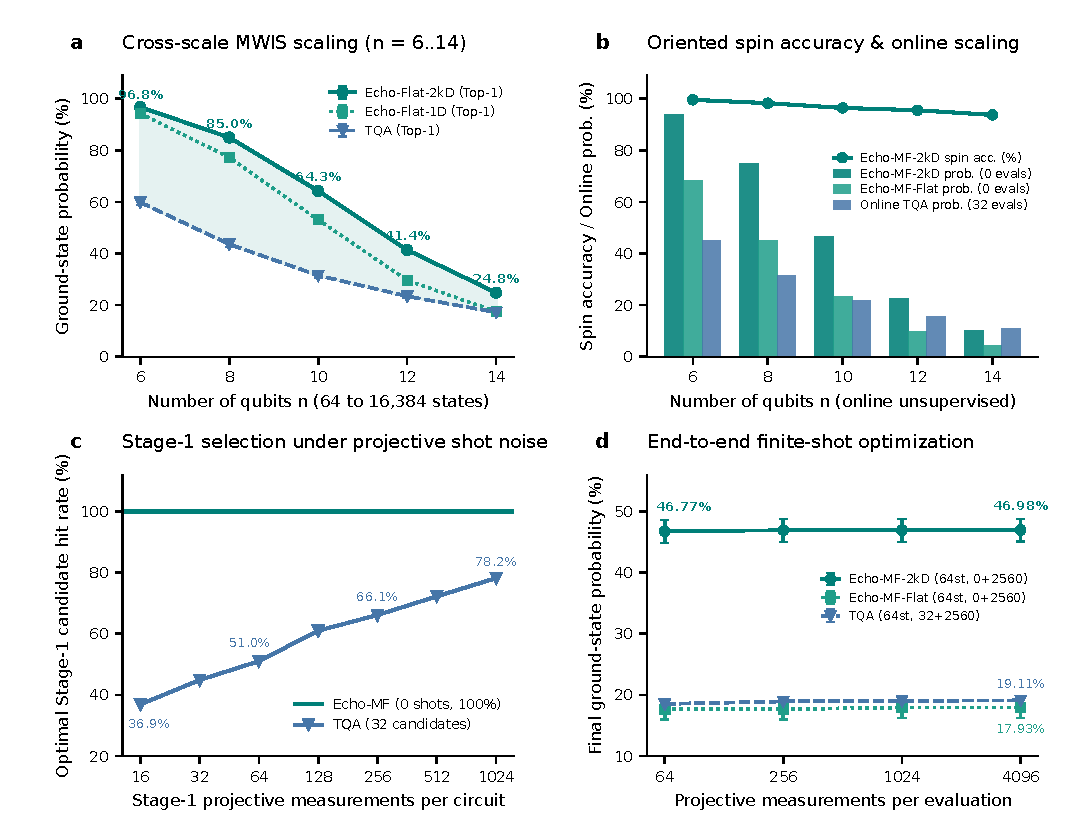
\includegraphics[width=0.92\textwidth]{figures/scale-and-shot-noise.pdf}
\vspace{-2pt}
\caption{\textbf{Cross-scale scaling across 5,120 MWIS test instances ($n \in \{6, 8, 10, 12, 14\}$) and immunity to projective measurement shot noise.} \textbf{a}, Uncapped equal-candidate (Top-1) offline scaling curves on MWIS at fixed depth $p = 10$ ($k = 5$ pairs) from $n = 6$ to $n = 14$ ($64$ to $16{,}384$ Hilbert-space dimensions, 1,024 unseen instances per scale) comparing \texttt{Echo-Flat-2kD}, \texttt{Echo-Flat-1D}, and \texttt{TQA}. \textbf{b}, Online training-free scaling on the exact same 5,120 instances showing oriented single-qubit spin accuracy (top curve) and zero-quantum-selection final ground-state probabilities of \texttt{Echo-MF-2kD} versus 32-evaluation online \texttt{TQA} and 1D \texttt{Echo-MF-Flat} (bottom bars). \textbf{c}, Stage-1 candidate selection shot-noise test ($n = 10, p = 10$, 1,024 instances) comparing \texttt{TQA}'s hit rate for selecting its noiseless optimal step size across $N_{\mathrm{shots}} \in \{16, 32, 64, 128, 256, 512, 1024\}$ against zero-quantum-measurement \texttt{Echo-MF} (identically $100\%$). \textbf{d}, End-to-end finite-shot parameter-shift variational optimization ($n = 10, p = 10$, 1,024 instances, 64 steps) across $N_{\mathrm{shots}} \in \{64, 256, 1024, 4096\}$. All error bars and shaded bands denote 4,000-resample bootstrap 95\% CIs.}
\label{fig:3}
\end{figure}

\begin{table}[!htbp]
\caption{\textbf{Cross-scale MWIS evaluation across $n \in \{6, 8, 10, 12, 14\}$ at fixed depth $p = 10$ (1,024 unseen test instances per scale; 5,120 instances total).} The left block reports offline uncapped equal-candidate (Top-1 and Top-2) final ground-state probabilities (\%) and paired net gains of \texttt{Echo-Flat-2kD} over \texttt{TQA}. The right block reports online training-free \texttt{Echo-MF-2kD} (0 Stage-1 quantum evaluations) and 1D \texttt{Echo-MF-Flat} versus online \texttt{TQA} (32 Stage-1 quantum evaluations) on the identical 5,120 instances, including single-qubit spin orientation accuracy, initial $\rightarrow$ final ground-state probabilities (\%), and mean Stage-2 gradient quantum calls. Bold denotes the best value in each comparison group.}
\label{tab:3}
\vspace{2pt}
\centering
\renewcommand{\arraystretch}{1.15}
\setlength{\tabcolsep}{3.5pt}
\resizebox{\textwidth}{!}{%
\begin{tabular}{cccccccccc}
\toprule
\shortstack[c]{\textbf{Size $n$} \\ \textbf{(Count)}} & \shortstack[c]{\textbf{Offline} \\ \textbf{\texttt{Echo-Flat-1D} (Top-1)}} & \shortstack[c]{\textbf{Offline \texttt{Echo-Flat-2kD}} \\ \textbf{(Top-1 / Top-2)}} & \shortstack[c]{\textbf{Offline \texttt{TQA}} \\ \textbf{(Top-1 / Top-2)}} & \shortstack[c]{\textbf{Offline \texttt{Echo-Flat-2kD} vs.} \\ \textbf{\texttt{TQA} (Top-1, pp)}} & \shortstack[c]{\textbf{Online \texttt{Echo-MF-2kD}} \\ \textbf{Spin Acc.}} & \shortstack[c]{\textbf{Online \texttt{Echo-MF-Flat}} \\ \textbf{(1D, 0 evals)}} & \shortstack[c]{\textbf{Online \texttt{Echo-MF-2kD}} \\ \textbf{($2k$-D, 0 evals)}} & \shortstack[c]{\textbf{Online \texttt{TQA}} \\ \textbf{(32 evals)}} & \shortstack[c]{\textbf{Stage-2 Quantum Calls} \\ \textbf{(\texttt{Echo-MF-2kD} / \texttt{TQA})}} \\
\midrule
$6$ ($1{,}024$) & $94.37^{+0.69}_{-0.73}$ & $\mathbf{96.79}^{+0.48}_{-0.53}\ /\ \mathbf{97.44}^{+0.39}_{-0.42}$ & $59.88^{+1.14}_{-1.13}\ /\ 62.18^{+1.15}_{-1.15}$ & $\mathbf{+36.91}\ ([+35.74, +38.02])$ & $99.61\%$ & $36.16 \rightarrow 68.49^{+2.34}_{-2.48}$ & $91.00 \rightarrow \mathbf{94.02}^{+0.96}_{-1.06}$ & $20.71 \rightarrow 45.19^{+1.15}_{-1.14}$ & $\mathbf{79.3}\ /\ 129.0$ \\
$8$ ($1{,}024$) & $77.25^{+1.36}_{-1.34}$ & $\mathbf{85.01}^{+0.92}_{-0.93}\ /\ \mathbf{87.18}^{+0.83}_{-0.81}$ & $43.62^{+1.07}_{-1.02}\ /\ 45.53^{+1.08}_{-1.04}$ & $\mathbf{+41.39}\ ([+40.10, +42.72])$ & $98.32\%$ & $15.96 \rightarrow 45.11^{+2.41}_{-2.40}$ & $69.41 \rightarrow \mathbf{74.99}^{+1.65}_{-1.68}$ & $12.07 \rightarrow 31.64^{+0.95}_{-0.93}$ & $\mathbf{68.6}\ /\ 121.7$ \\
$10$ ($1{,}024$) & $53.08^{+1.51}_{-1.57}$ & $\mathbf{64.29}^{+1.22}_{-1.24}\ /\ \mathbf{67.41}^{+1.13}_{-1.14}$ & $31.52^{+0.82}_{-0.84}\ /\ 33.06^{+0.86}_{-0.90}$ & $\mathbf{+32.76}\ ([+31.35, +34.17])$ & $96.45\%$ & $5.39 \rightarrow 23.23^{+1.83}_{-1.92}$ & $42.20 \rightarrow \mathbf{46.70}^{+1.78}_{-1.90}$ & $6.81 \rightarrow 21.94^{+0.68}_{-0.68}$ & $\mathbf{63.6}\ /\ 121.0$ \\
$12$ ($1{,}024$) & $29.64^{+1.33}_{-1.25}$ & $\mathbf{41.41}^{+1.18}_{-1.15}\ /\ \mathbf{45.51}^{+1.10}_{-1.11}$ & $23.45^{+0.69}_{-0.66}\ /\ 24.48^{+0.69}_{-0.67}$ & $\mathbf{+17.96}\ ([+16.75, +19.16])$ & $95.57\%$ & $1.26 \rightarrow 9.74^{+1.21}_{-1.12}$ & $21.38 \rightarrow \mathbf{22.64}^{+1.31}_{-1.38}$ & $3.88 \rightarrow 15.55^{+0.54}_{-0.50}$ & $\mathbf{62.6}\ /\ 119.6$ \\
$14$ ($1{,}024$) & $17.47^{+0.96}_{-0.96}$ & $\mathbf{24.84}^{+0.95}_{-0.93}\ /\ \mathbf{27.86}^{+0.95}_{-0.91}$ & $17.23^{+0.58}_{-0.53}\ /\ 18.16^{+0.62}_{-0.57}$ & $\mathbf{+7.61}\ ([+6.66, +8.57])$ & $93.75\%$ & $0.46 \rightarrow 4.32^{+0.70}_{-0.66}$ & $\mathbf{10.12} \rightarrow 10.13^{+0.93}_{-0.90}$ & $2.17 \rightarrow \mathbf{10.94}^{+0.44}_{-0.40}$ & $\mathbf{61.3}\ /\ 119.8$ \\
\bottomrule
\end{tabular}%
}
\end{table}
Evaluating 5,120 unseen MWIS test instances across $n \in \{6, 8, 10, 12, 14\}$ at fixed depth $p = 10$ ($2k = 10$ manifold parameters) reveals how $2k$-dimensional refinement reshapes scaling in the overcomplete $n > 2k$ regime (Figure 3a, b and Table 3). In offline equal-candidate comparisons (Table 3, left), 1D \texttt{Echo-Flat-1D (Top-1)} suffers severe Diophantine frequency crowding once $n \ge 12 > 2k$, with initial product probabilities dropping to $3.69\%$ ($n=12$) and $1.29\%$ ($n=14$). Unlocking all $2k=10$ intra-pair degrees of freedom in \texttt{Echo-Flat-2kD} boosts initial product probabilities by $6.2\mbox{--}8.6\times$ in the overcomplete regime (to $22.87\%$ at $n=12$ and $11.08\%$ at $n=14$). After Stage-2 recoupling, \texttt{Echo-Flat-2kD (Top-1)} outperforms both \texttt{TQA (Top-1)} and \texttt{Echo-Flat-1D (Top-1)} across all five system sizes with paired net gains over \texttt{TQA} of $\mathbf{+36.91}, \mathbf{+41.39}, \mathbf{+32.76}, \mathbf{+17.96}$, and $\mathbf{+7.61}$ pp (reaching Top-1 / Top-2 probabilities of $\mathbf{64.29}\% / \mathbf{67.41}\%$, $\mathbf{41.41}\% / \mathbf{45.51}\%$, and $\mathbf{24.84}\% / \mathbf{27.86}\%$ at $n=10, 12, 14$; all 95\% CIs strictly positive).

In online training-free mode (Table 3, right), 1D soft-marginal overlap decoding (\texttt{Echo-MF-Flat}) outperforms \texttt{TQA} at $n \le 10$ but collapses at $n=12, 14$ ($9.74\%, 4.32\%$) as unoriented soft marginals compound 1D frequency crowding. Conversely, temperature-continuation cluster orientation in \texttt{Echo-MF-2kD} sustains $93.75\%\mbox{--}99.61\%$ single-qubit orientation accuracy across all 5,120 instances. With zero Stage-1 measurements, \texttt{Echo-MF-2kD} achieves final probabilities of $\mathbf{94.02}\%, \mathbf{74.99}\%, \mathbf{46.70}\%, \mathbf{22.64}\%$ across $n=6, 8, 10, 12$---beating 32-evaluation online \texttt{TQA} by $\mathbf{+48.83}, \mathbf{+43.35}, \mathbf{+24.76}, \mathbf{+7.09}$ pp while cutting Stage-2 quantum gradient calls roughly in half ($\mathbf{61.3\mbox{--}79.3}$ versus $119.6\mbox{--}129.0$). At $n=14$, where large conflict penalties ($Q = 2\max_i v_i$) steepen excited-state energy barriers, \texttt{Echo-MF-2kD}'s zero-measurement Stage-1 classical product state ($\mathbf{10.12}\%$, $4.7\times$ \texttt{TQA}'s initial $2.17\%$ and $22\times$ \texttt{Echo-MF-Flat}'s $0.46\%$) already matches the final post-optimization probability of online \texttt{TQA} ($10.94\%$).

This mechanistic scaling extends across the five canonical Ising benchmark families (\texttt{MWIS}, \texttt{Dense Ising}, \texttt{Sparse Ising}, \texttt{Grid Ising}, and \texttt{Pinned MaxCut}\citep{yao2026echo}) in uncapped $n=11, 12$ ($p=10$, 500 instances) boundary experiments (Extended Data Table 1). \texttt{Echo-Flat-2kD} yields $+12.05$ and $+10.57$ pp gains over \texttt{Echo-Flat-1D} on heterogeneous-field \texttt{MWIS} ($\mathbf{56.69}\%$ and $\mathbf{41.66}\%$, beating \texttt{TQA} by $\mathbf{+28.81}$ and $\mathbf{+16.56}$ pp), elevates Stage-1 initial product probabilities on zero-mean Gaussian \texttt{Dense}, \texttt{Sparse}, and \texttt{Grid Ising} from $5.05\%\mbox{--}9.12\%$ (\texttt{Echo-Flat-1D}) to $24.70\%\mbox{--}37.47\%$, and surpasses online \texttt{TQA} across all four non-zero-field families. Conversely, on the negative-control family \texttt{Pinned MaxCut} where interior local fields vanish identically ($h_i = 0$), both 1D and $2k$D initial probabilities remain strictly bounded by $2^{-n_0}$ ($0.20\%\mbox{--}0.37\%$), confirming our theoretical premise that complete spin-echo pair evolution is driven specifically by non-vanishing local external fields $H_h$.


\subsection*{Shot-noise immunity and early-stopping efficiency}

Under realistic quantum hardware execution, projective measurements introduce multinomial shot noise of scale $O(N_{\mathrm{shots}}^{-1/2})$ into every energy evaluation. Across all 1,024 held-out MWIS center test instances ($n=10, p=10$), online \texttt{TQA} suffers severe Stage-1 misselection ("Winner's Curse") when picking the lowest empirical energy among its 32 candidate step sizes (Figure 3c and Extended Data Table 2): at $N_{\mathrm{shots}} = 16, 32, 64$, statistical fluctuations limit \texttt{TQA}'s noiseless-optimum hit rate to $36.86\%, 44.86\%, 51.02\%$, reaching only $78.20\%$ at $N_{\mathrm{shots}} = 1024$. Because \texttt{Echo-MF-2kD} and \texttt{Echo-MF-Flat} execute Stage-1 manifold refinement deterministically on a classical processor with zero quantum measurements, their Stage-1 candidate selection is $100\%$ immune to shot noise across all shot budgets.

When both Stage-1 selection and 64-step Stage-2 parameter-shift gradient optimization ($2 \times 2p = 40$ circuit executions per step) operate under finite measurement shots $N_{\mathrm{shots}} \in \{64, 256, 1024, 4096\}$, \texttt{Echo-MF-2kD} achieves substantial measurement savings and noise resilience (Figure 3d and Extended Data Table 2). With zero quantum measurements (0 steps), \texttt{Echo-MF-2kD}'s classical product initial state ($\mathbf{42.20}^{+1.55}_{-1.70}\%$) already exceeds $2.2\times$ the final probability of 64-step noisy \texttt{TQA} ($18.52\%\mbox{--}19.11\%$ after $2{,}592$ circuit evaluations). With early stopping at 16 steps ($640$ evaluations, saving $75.3\%$ of shots) and 32 steps ($1{,}280$ evaluations, saving $50.6\%$ of shots), \texttt{Echo-MF-2kD} reaches $44.03\%\mbox{--}44.73\%$ and $45.60\%\mbox{--}46.28\%$, outperforming 64-step \texttt{TQA} by $\mathbf{+25.51\mbox{--}{+}25.62}$ pp and $\mathbf{+27.08\mbox{--}{+}27.20}$ pp. At 64 steps ($2{,}560$ evaluations), \texttt{Echo-MF-2kD} reaches $\mathbf{46.77}\%\mbox{--}\mathbf{46.98}\%$, a paired net gain of $\mathbf{+27.87\mbox{--}{+}28.25}$ pp over \texttt{TQA}.


\section*{Discussion}

By proving that exact spin-echo parity cancellation of quadratic couplings $H_J$ extends from a 1D scalar ray to the entire $2k$-dimensional complete-pair submanifold inside the unmodified depth-$2k$ global QAOA circuit, this work establishes an exact equivalence between multi-body quantum expected energy and classical product-state energy: $\langle\psi_p(\boldsymbol{g},\boldsymbol{\theta})|H_C|\psi_p(\boldsymbol{g},\boldsymbol{\theta})\rangle \equiv E_{\mathrm{prod}}(\boldsymbol{g},\boldsymbol{\theta})$. This structural insight resolves the long-standing tension between hardware-native circuit execution and site-specific phase initialization. Rather than modifying the quantum circuit ansatz with site-customized mixers \citep{egger2021warm,tate2023warm} or expending online quantum evaluations on homogeneous annealing grids \citep{sack2021quantum}, \texttt{Echo-MF-2kD} exploits the hidden integrable $2k$-dimensional product submanifold to align heterogeneous single-qubit phases and suppress effective-field inversions purely on a classical processor before launching full-angle quantum entanglement optimization.

Beyond QAOA, our three-stage division of labor---classical mean-field topological orientation, exact adjoint control on an embedded symmetry-decoupled product manifold, and symmetry-breaking multi-body recoupling \citep{dupont2022entanglement}---provides a general methodological blueprint for parameterized quantum circuits and many-body variational simulation. Whenever a target Hamiltonian decomposes into terms of opposite parity under a global hardware-native symmetry operation (such as global Pauli flips in spin lattices or particle-hole conjugation in fermionic systems), inserting symmetry pivots carves out a classically tractable low-dimensional submanifold within the deep variational ansatz. Pre-optimizing classical surrogate energies and local stability guards on this exact submanifold via $O(kn)$ reverse-mode $\mathrm{SU}(2)$ adjoint differentiation avoids barren plateaus and shot-noise misselection while reducing classical preprocessing from $O(n^{3.5})$ semidefinite programming to sparse-graph linear complexity $O(T_{\mathrm{mf}}|E| + kn)$.

Our theoretical assumptions and cross-family experiments also delineate two clear operational boundaries. First, because single-qubit phase evolution $e^{-2i g_j H_h}$ on the complete Echo-pair submanifold is generated exclusively by local external fields $H_h$, problems with identically zero local fields ($h = 0$, such as unweighted MaxCut or interior vertices of \texttt{Pinned MaxCut}) experience no phase differentiation on the pure Echo manifold; extending \texttt{Echo-MF-2kD} to field-free graphs requires pinning a reference vertex or applying a single mean-field symmetry-breaking layer to induce effective local fields. Second, when system size scales into the deep overcomplete regime ($n = 14 > 2k = 10$) under large constraint penalties ($Q = 2\max_i v_i$), although \texttt{Echo-MF-2kD}'s zero-measurement Stage-1 product state ($10.12\%$) matches the final post-optimization probability of online \texttt{TQA} ($10.94\%$), Stage-2 optimization of the expected energy $\langle H_C \rangle$ prioritizes suppressing high-penalty excited tails over amplifying the ground-state peak ($10.12\% \rightarrow 10.13\%$). Replacing the Stage-2 expected-energy objective with tail-focused Conditional Value-at-Risk (CVaR) objectives or scaling circuit depth proportionally with system size ($p \propto n$) on neutral Rydberg atom arrays offers a direct path to hundred-qubit constrained quantum optimization.


\section*{Methods}

\subsection*{Problem Formulation and Theoretical Preliminaries}

\textbf{Normalized Ising Hamiltonian and standard global QAOA ansatz.} We consider an $n$-qubit Ising energy function with local external fields over spin configurations $s \in \{-1, +1\}^n$ (mapped to binary variables via $x_i = (1 + s_i)/2 \in \{0, 1\}$):
\[
E(s) = \frac{1}{2}s^\top J s + h^\top s + C, \qquad s \in \{-1, +1\}^n,
\]
where $J \in \mathbb{R}^{n \times n}$ is symmetric with zero diagonal and $h \in \mathbb{R}^n$ is the local external field vector. To standardize energy scales across problem families and graph sizes without altering configuration ordering or energy gap ratios, raw coefficients $(J_{\mathrm{raw}}, h_{\mathrm{raw}}, C_{\mathrm{raw}})$ are normalized by the per-qubit root-mean-square (RMS) scale factor $\lambda = \sqrt{(\|J_{\mathrm{raw}}\|_F^2 + \|h_{\mathrm{raw}}\|_2^2)/n}$ to yield $J = J_{\mathrm{raw}}/\lambda$, $h = h_{\mathrm{raw}}/\lambda$, and $C = 0$, satisfying $(\|J\|_F^2 + \|h\|_2^2)/n = 1$. In the $2^n$-dimensional Hilbert space with computational basis states $|s\rangle$ and diagonal spin operators $S_i = \operatorname{diag}(-1, +1) = -Z_i$, the problem Hamiltonian is $H_C = H_J + H_h$, where $H_J = \sum_{1 \le i < j \le n} J_{ij} S_i S_j$ and $H_h = \sum_{i=1}^n h_i S_i$. A depth-$p$ standard global QAOA circuit applies alternating cost unitaries $U_C(\gamma_\ell) = e^{-i\gamma_\ell H_C}$ and global transverse-field mixer unitaries $U_B(\beta_\ell) = e^{-i\beta_\ell \sum_{i=1}^n X_i}$ to the uniform superposition $|+\rangle^{\otimes n}$, preparing $|\psi_p(\vartheta)\rangle = U_B(\beta_p)U_C(\gamma_p)\cdots U_B(\beta_1)U_C(\gamma_1)|+\rangle^{\otimes n}$ parameterized by $\vartheta = (\gamma_1, \ldots, \gamma_p, \beta_1, \ldots, \beta_p) \in [-10\pi, 10\pi]^p \times [-\pi/2, \pi/2)^p$.

\textbf{Complete spin-echo pair decoupling on the $2k$-dimensional submanifold.} Define the global spin-flip parity operator $F = \prod_{i=1}^n X_i$, which satisfies $F^\dagger = F$, $F^2 = I$, $F|s\rangle = |-s\rangle$, and $U_B(\pi/2) = (-i)^n F$. Under conjugation by $F$, the quadratic coupling and local field operators obey opposite parity relations:
\[
F H_J F = H_J, \qquad F H_h F = -H_h.
\]
For any positive even circuit depth $p = 2k$ ($k \ge 1$), we partition the $2k$ layers into $k$ adjacent \emph{complete spin-echo pairs} ($j = 1, \ldots, k$) by assigning anti-symmetric cost angles $(\gamma_{2j-1}, \gamma_{2j}) = (-g_j, g_j)$ and mixer angles $(\beta_{2j-1}, \beta_{2j}) = (\pi/2, \theta_j)$ \citep{yao2026echo}. Because $H_C$ and $F H_C F$ are diagonal in the computational basis and commute ($[H_C, F H_C F] = 0$), the composite two-layer unitary of the $j$-th pair simplifies identically (up to the global phase $(-i)^n$) to
\[
E(g_j, \theta_j) = U_B(\theta_j) e^{-i g_j H_C} F e^{i g_j H_C} = U_B(\theta_j) e^{-i g_j (H_J + H_h)} e^{i g_j (F H_J F + F H_h F)} F = U_B(\theta_j) e^{-2i g_j H_h} F.
\]
Because $H_J$ cancels identically within each pair for any $(g_j, \theta_j) \in \mathbb{R}^2$, the $2p$-layer circuit unitary across the entire $2k$-dimensional complete-pair submanifold $(\boldsymbol{g}, \boldsymbol{\theta}) = (g_1, \ldots, g_k, \theta_1, \ldots, \theta_k) \in \mathbb{R}^k \times \mathbb{R}^k$ decomposes into single-qubit operators, preparing the exact product state $|\psi_p(\boldsymbol{g}, \boldsymbol{\theta})\rangle = \bigotimes_{i=1}^n u_i^{(k)}(\boldsymbol{g}, \boldsymbol{\theta})$. In the single-qubit basis $(|s_i = -1\rangle, |s_i = +1\rangle)$ starting from $u_i^{(0)} = \frac{1}{\sqrt{2}}(1, 1)^\top$, the spinor $u_i^{(j)} = (u_{i,-}^{(j)}, u_{i,+}^{(j)})^\top$ evolves across $j = 1, \ldots, k$ via the $2 \times 2$ unitary recursion
\[
\binom{u_{i,-}^{(j)}}{u_{i,+}^{(j)}} = M(\theta_j)\binom{e^{2i g_j h_i} u_{i,+}^{(j-1)}}{e^{-2i g_j h_i} u_{i,-}^{(j-1)}}, \qquad M(\theta_j) = \begin{pmatrix} \cos\theta_j & -i\sin\theta_j \\ -i\sin\theta_j & \cos\theta_j \end{pmatrix}.
\]
\textbf{Exact quantum--classical product-energy identity and first-order Stage-2 recoupling.} Denoting the terminal positive-spin probability of qubit $i$ by $p_i^+(\boldsymbol{g}, \boldsymbol{\theta}) = |u_{i,+}^{(k)}|^2$ and its magnetization by $m_i(\boldsymbol{g}, \boldsymbol{\theta}) = 2p_i^+(\boldsymbol{g}, \boldsymbol{\theta}) - 1 = |u_{i,+}^{(k)}|^2 - |u_{i,-}^{(k)}|^2 \in [-1, 1]$, the probability of measuring any target configuration $s^\star \in \{-1, +1\}^n$ is $P(s^\star) = \prod_{i=1}^n \frac{1 + s_i^\star m_i}{2}$. Because distinct qubits are unentangled on the $2k$-dimensional submanifold, two-body spin correlations factorize exactly ($\langle\psi_p(\boldsymbol{g}, \boldsymbol{\theta})| S_i S_j |\psi_p(\boldsymbol{g}, \boldsymbol{\theta})\rangle = m_i m_j$ for all $i \ne j$), yielding the exact operator expectation identity $\langle\psi_p(\boldsymbol{g}, \boldsymbol{\theta})| H_C |\psi_p(\boldsymbol{g}, \boldsymbol{\theta})\rangle \equiv E_{\mathrm{prod}}(\boldsymbol{g}, \boldsymbol{\theta}) = \frac{1}{2}\boldsymbol{m}^\top J\boldsymbol{m} + \boldsymbol{h}^\top\boldsymbol{m} + C$. When Stage-2 optimization perturbs the $j$-th pair's cost angles along the symmetry-breaking direction $(\gamma_{2j-1}, \gamma_{2j}) = (-g_j + \delta_j, g_j + \delta_j)$, commuting $F$ through $e^{i(g_j + \delta_j)H_C}$ yields $E(g_j, \theta_j; \delta_j) = U_B(\theta_j) e^{-2i\delta_j H_J} e^{-2i g_j H_h} F$, which re-activates the quadratic coupling generator $-2i H_J$ linearly at $O(\delta_j)$.


\subsection*{Module Design and Algorithmic Procedure}

\textbf{Damped mean-field inference and temperature-continuation cluster orientation.} Given an unseen instance $(J, h)$ in online mode, Stage 1 first estimates soft spin polarizations by running $T_{\mathrm{mf}}$ damped mean-field iterations \citep{wainwright2008graphical} with damping factor $\alpha_{\mathrm{d}} \in (0, 1)$ at a characteristic inverse temperature $\beta_{\mathrm{mf}}^\star > 0$ from $\boldsymbol{m}^{(0)} = \mathbf{0}$:
\[
m_i^{(t)} = (1 - \alpha_{\mathrm{d}}) m_i^{(t-1)} + \alpha_{\mathrm{d}} \tanh\!\left[-\beta_{\mathrm{mf}}^\star\left(h_i + \sum_{j=1}^n J_{ij} m_j^{(t-1)}\right)\right], \qquad \pi_i^{\mathrm{mf}} = \frac{1 + m_i^{(T_{\mathrm{mf}})}}{2}.
\]
While 1D \texttt{Echo-MF-Flat} decodes $\boldsymbol{\pi}^{\mathrm{mf}}$ directly via 1D distribution overlap $S(a) = \prod_{i=1}^n [\pi_i^{\mathrm{mf}} q_i(a) + (1 - \pi_i^{\mathrm{mf}})(1 - q_i(a))]$ \citep{yao2026echo}, soft marginals on frustrated edges can remain near $0.5$ and pull multi-scalar optimization toward conflicting basins. To lock onto a self-consistent binary target orientation $\hat{\boldsymbol{s}} \in \{-1, +1\}^n$ deterministically, we construct a candidate seed pool from $2\boldsymbol{\pi}^{\mathrm{mf}} - \mathbf{1}$ and single-spin flips on the most uncertain qubits, propagate each seed through damped mean-field updates across an ascending inverse-temperature schedule $\beta_1 < \beta_2 < \beta_3$, and apply zero-temperature greedy single-spin flips and adjacent conflicting-edge $(i, j)$ two-spin swaps that strictly decrease the classical Ising energy $\frac{1}{2}\boldsymbol{s}^\top J\boldsymbol{s} + \boldsymbol{h}^\top\boldsymbol{s}$, selecting the lowest-energy self-consistent orientation $\hat{\boldsymbol{s}}$.

\textbf{1D Daubechies maximally flat anchors and zero-free interval convexity.} To initialize optimization on the $2k$-dimensional submanifold, we extract resonance anchors along the 1D Daubechies maximally flat ray $\boldsymbol{g}(a) = a \boldsymbol{r}^{\mathrm{flat}}$ with dyadic ratio $\boldsymbol{r}^{\mathrm{flat}} = (1, 2, \ldots, 2)$ and pre-synthesized maximally flat even-layer mixer angles $\boldsymbol{\theta}^{\mathrm{flat}} \in [-\pi/2, \pi/2)^k$ obtained via Daubechies spectral factorization and two-channel lattice reduction \citep{daubechies1988orthonormal,herrmann1971approximation,yao2026echo}. Under this 1D response, single-qubit positive-spin probability is given by the regularized incomplete Beta function $p_k(q) = I_q(k, k) = q^k \sum_{r=0}^{k-1} \binom{k-1+r}{r}(1-q)^r$ with $q = (1 + \sin(4a h_i))/2$. For any target orientation $\hat{\boldsymbol{s}} \in \{-1, +1\}^n$, let $w_i = 4h_i \hat{s}_i$ and phase error $e_i(a) = \operatorname{wrap}_{(-\pi, \pi]}(a w_i - \pi/2)$. Because the single-qubit negative log-likelihood $\ell_k(e) = -\ln p_k((1 + \cos e)/2)$ has a strictly increasing first derivative on $(-\pi, \pi)$ governed by the log-concave kernel $\sin^{2k-1}v$, the 1D negative log-likelihood $\mathcal{L}_k(a) = \sum_{i=1}^n \ell_k(e_i(a))$ is \emph{strictly convex} in $a$ on every open interval bounded by the adjacent zero-probability singularities $a = (-\pi/2 + 2\pi z)/w_i$ ($z \in \mathbb{Z}$). Enumerating all singularity breakpoints on $[-G, G]$ and applying deterministic derivative bisection within each zero-free open interval extracts the top $M_{\mathrm{anc}}$ separated minima $a^{(m)}$, defining initial manifold anchors $(\boldsymbol{g}^{(0,m)}, \boldsymbol{\theta}^{(0)}) = (a^{(m)}\boldsymbol{r}^{\mathrm{flat}}, \boldsymbol{\theta}^{\mathrm{flat}})$.

\textbf{Composite physical objective and exact $O(kn)$ reverse-mode $\mathrm{SU}(2)$-adjoint refinement.} Denote the active non-zero-field qubit set by $NZ = \{i : h_i \ne 0\}$, the target-direction spin probability by $\pi_i(\boldsymbol{g}, \boldsymbol{\theta}) = p_i^+(\boldsymbol{g}, \boldsymbol{\theta})^{\mathbf{1}[\hat{s}_i=+1]}(1 - p_i^+(\boldsymbol{g}, \boldsymbol{\theta}))^{\mathbf{1}[\hat{s}_i=-1]}$, and the local effective field by $h_i^{\mathrm{eff}}(\boldsymbol{m}) = h_i + (J\boldsymbol{m})_i$. To prioritize qubits subject to strong effective drives and prevent Stage-2 local field inversions, we define normalized flip-sensitivity weights $w_i = 1 + \kappa_w |h_i + (J\hat{\boldsymbol{s}})_i| / (\frac{1}{|NZ|}\sum_{j \in NZ} |h_j + (J\hat{\boldsymbol{s}})_j|)$ and formulate the composite manifold objective
\[
\begin{aligned}
\mathcal{L}(\boldsymbol{g}, \boldsymbol{\theta}) ={}& -\sum_{i \in NZ} w_i \ln \pi_i(\boldsymbol{g}, \boldsymbol{\theta}) + \lambda_{\mathrm{quad}} \sum_{i \in NZ} w_i \operatorname{softplus}\!\big(\tau_{\mathrm{quad}}(\pi_{\mathrm{safe}} - \pi_i(\boldsymbol{g}, \boldsymbol{\theta}))\big) \\
&+ \frac{\lambda_{\mathrm{inv}}}{\tau_{\mathrm{inv}}} \sum_{i \in NZ} \operatorname{softplus}\!\big(\tau_{\mathrm{inv}}(\hat{s}_i h_i^{\mathrm{eff}}(\boldsymbol{m}) + \delta_{\mathrm{inv}})\big) + \alpha_E E_{\mathrm{prod}}(\boldsymbol{g}, \boldsymbol{\theta}) \\
&+ \frac{\mu_g}{2}\|\boldsymbol{g} - \boldsymbol{g}^{(0)}\|_2^2 + \frac{\mu_\theta}{2}\|\boldsymbol{\theta} - \boldsymbol{\theta}^{(0)}\|_2^2.
\end{aligned}
\]
Here, the first two terms drive all active qubits into the correct target hemisphere above safety margin $\pi_{\mathrm{safe}} > 0.5$; the third term is the \emph{local effective-field inversion guard}, which penalizes states where $\hat{s}_i h_i^{\mathrm{eff}}(\boldsymbol{m}) > -\delta_{\mathrm{inv}}$ so that each spin remains energetically aligned against its local effective field upon Stage-2 coupling activation; the fourth term minimizes the exact classical product energy $E_{\mathrm{prod}}$; and the final two terms regularize deviations from the Daubechies anchor $(\boldsymbol{g}^{(0)}, \boldsymbol{\theta}^{(0)})$.

Exact gradients $\nabla_{(\boldsymbol{g}, \boldsymbol{\theta})}\mathcal{L}$ are computed in $O(kn + n^2)$ operations via reverse-mode $\mathrm{SU}(2)$-adjoint differentiation. Initializing the terminal adjoint spinor $\bar{u}_i^{(k)} = \frac{\partial\mathcal{L}}{\partial u_i^{(k)*}} = (0,\ \frac{\partial\mathcal{L}}{\partial p_i^+} u_{i,+}^{(k)})^\top$ from $\frac{\partial E_{\mathrm{prod}}}{\partial p_i^+} = 2 h_i^{\mathrm{eff}}(\boldsymbol{m})$ and $\frac{\partial\pi_i}{\partial p_i^+} = \hat{s}_i$, and denoting the post-phase intermediate spinor at pair $j$ by $\tilde{u}_i^{(j)} = (e^{2i g_j h_i} u_{i,+}^{(j-1)},\ e^{-2i g_j h_i} u_{i,-}^{(j-1)})^\top$, backward recursion from $j = k$ down to $j = 1$ yields
\[
\frac{\partial\mathcal{L}}{\partial\theta_j} = \mu_\theta(\theta_j - \theta_j^{(0)}) + 2\operatorname{Re}\sum_{i=1}^n \big(\bar{u}_i^{(j)}\big)^\dagger \frac{d M(\theta_j)}{d\theta_j} \tilde{u}_i^{(j)}, \qquad \tilde{\bar{u}}_i^{(j)} = M(\theta_j)^\dagger \bar{u}_i^{(j)},
\]
\[
\frac{\partial\mathcal{L}}{\partial g_j} = \mu_g(g_j - g_j^{(0)}) + 2\operatorname{Re}\sum_{i=1}^n 2i h_i \Big[\big(\tilde{\bar{u}}_{i,-}^{(j)}\big)^* \tilde{u}_{i,-}^{(j)} - \big(\tilde{\bar{u}}_{i,+}^{(j)}\big)^* \tilde{u}_{i,+}^{(j)}\Big], \qquad \binom{\bar{u}_{i,-}^{(j-1)}}{\bar{u}_{i,+}^{(j-1)}} = \binom{e^{2i g_j h_i} \tilde{\bar{u}}_{i,+}^{(j)}}{e^{-2i g_j h_i} \tilde{\bar{u}}_{i,-}^{(j)}}.
\]
To prevent even-layer mixers from degenerating into pure spin flips ($|\theta_j| \to \pi/2$, which would freeze transverse mixing in Stage 2), we enforce the non-degenerate mixer bound $|\theta_j| \le \theta_{\max} < \pi/2$ and trust-region box constraints around each anchor. Refinement proceeds in two stages: Step 1a optimizes the $k$ cost angles $\boldsymbol{g}$ with $\boldsymbol{\theta} = \boldsymbol{\theta}^{(0)}$ fixed; when $|NZ| > k$, Step 1b jointly optimizes all $2k$ parameters $(\boldsymbol{g}, \boldsymbol{\theta})$. Across refined anchors, the candidate minimizing $E_{\mathrm{prod}}$ with maximum all-qubit quadrant satisfaction is expanded into the $2p$-dimensional starting point $\vartheta_0$.


\subsection*{Experimental Protocol and Evaluation Setup}

\textbf{Benchmark datasets and controlled instance verification.} Experiments are conducted on two verified benchmark suites sharing RMS normalization and exact two-step unique-ground-state verification:

\begin{enumerate}\setlength{\itemsep}{1pt}\setlength{\parskip}{1pt}\setlength{\topsep}{2pt}
\item \emph{MWIS learning and cross-scale benchmark (\texttt{data/mwis})}: Connected sparse graphs (Hamiltonian cycle plus random edges with expected degree $3$, vertex weights $v_i \sim \mathcal{U}(0.5, 1.5)$, and conflict penalty $Q = 2\max_i v_i$ guaranteeing that all local and global energy minima are valid independent sets). The center $n = 10$ dataset comprises 4,096 training, 512 validation, and 1,024 held-out test instances evaluated across $p \in \{8, 10, 12\}$ ($k \in \{4, 5, 6\}$). Large-sample cross-scale generalization is evaluated at fixed depth $p = 10$ across $n \in \{6, 8, 10, 12, 14\}$ with 1,024 unseen test instances per scale (5,120 test instances total, spanning $64$ to $16{,}384$ Hilbert-space dimensions).
\item \emph{Five-family Ising benchmark (\texttt{data/benchmark})}: Encompasses \texttt{Dense Ising}, \texttt{Sparse Ising}, \texttt{Grid Ising}, \texttt{MWIS}, and \texttt{Pinned MaxCut} (50 instances per family per size across $n = 6\ldots 16$, 2,750 instances total, including the 500-instance uncapped mechanistic boundary suite at $n \in \{11, 12\}, p = 10$).

\end{enumerate}
\textbf{Baseline fairness and two-stage evaluation protocol.} All compared methods are evaluated under a unified two-stage protocol (Stage-1 initialization $\rightarrow$ Stage-2 continuous full-angle optimization). In online training-free comparisons (Table 2 and Table 3 right), every initializer receives exclusively $(J, h)$ with zero training data: \texttt{RI (1)} samples a single random starting point ($0$ Stage-1 evaluations); \texttt{RI (32)} and online \texttt{TQA} ($\gamma_\ell = \Delta t(\ell - 0.5)/p$, $\beta_\ell = -\Delta t(1 - (\ell - 0.5)/p)$) evaluate 32 candidates on the quantum circuit objective $\langle H_C \rangle$ to select the lowest-energy start ($32$ Stage-1 quantum evaluations); \texttt{Echo-Energy}, \texttt{Echo-MF-Alt}, \texttt{Echo-MF-End}, and \texttt{Echo-MF-Flat} scan 128 uniform scalar points on $[-10\pi, 10\pi]$ classically ($0$ Stage-1 quantum evaluations); and \texttt{Echo-MF-2kD} performs staged $2k$-dimensional adjoint refinement ($0$ Stage-1 quantum evaluations). All Stage-1 starting points $\vartheta_0 \in \mathbb{R}^{2p}$ are passed to the identical Stage-2 L-BFGS-B quantum energy optimizer, returning the lowest-energy evaluated point $\vartheta_{\mathrm{best}}$ for independent ground-state probability scoring $P_{\mathrm{gs}} = |\langle s^\star | \psi_p(\vartheta_{\mathrm{best}}) \rangle|^2$. In offline equal-candidate comparisons (Table 1 top and Table 3 left), \texttt{Echo-Flat-2kD}, \texttt{Echo-Flat-1D}, and \texttt{TQA} are compared under strictly matched candidate budgets (\texttt{Top-1} and \texttt{Top-2}) without wall-clock truncation.

\textbf{Finite-shot projective noise and statistical inference.} Shot-noise experiments on the 1,024-instance $n = 10, p = 10$ MWIS test set evaluate both Stage-1 candidate selection under multinomial projective sampling (Regime A, $N_{\mathrm{shots}} \in \{16, 32, 64, 128, 256, 512, 1024\}$, 5 independent trials per instance) and end-to-end noisy variational optimization (Regime B, Stage-1 noisy selection followed by 64 steps of parameter-shift gradient descent requiring $2 \times 2p = 40$ circuit executions per step across $N_{\mathrm{shots}} \in \{64, 256, 1024, 4096\}$). All reported means and paired net differences across the manuscript are accompanied by 95\% confidence intervals computed via instance-level non-parametric percentile bootstrap (\texttt{replicates = 4,000}).


\subsection*{Implementation Details}

All hyperparameters of \texttt{Echo-MF-2kD} (\texttt{Echo-Flat-2kD}) were locked on the $n = 10$ validation set (512 instances) and frozen zero-shot across all test sets, depths, and system sizes. In Stage 1, damped mean-field inference uses $T_{\mathrm{mf}} = 80$, $\alpha_{\mathrm{d}} = 0.5$, and $\beta_{\mathrm{mf}}^\star = 2.0$; deterministic temperature-continuation cluster orientation (\texttt{resolve\_\allowbreak{}prior\_\allowbreak{}direction}) perturbs up to $\min(n, 6)$ most uncertain spins (closest to $\pi_i^{\mathrm{mf}} = 0.5$), runs 28 damped updates ($\alpha_{\mathrm{d}} = 0.5$) at each inverse temperature $\beta \in \{2.5, 6.0, 16.0\}$, and performs up to $2n$ zero-temperature single-spin and conflicting-edge swap sweeps. Daubechies Flat-Top synthesis uses extended-precision arithmetic (\texttt{mpmath}, $40 + 3k$ decimal digits, construction residuals $< 10^{-10}$), and 1D convex-interval bisection runs up to 60 steps (tolerance $10^{-9}$) per zero-free interval to extract $M_{\mathrm{anc}} = 10$ anchors. In the composite adjoint objective, weights are fixed at $\kappa_w = 1.5$, $\lambda_{\mathrm{quad}} = 0.5$, $\tau_{\mathrm{quad}} = 14.0$, $\pi_{\mathrm{safe}} = 0.56$, $\lambda_{\mathrm{inv}} = 1.5$, $\tau_{\mathrm{inv}} = 10.0$, $\delta_{\mathrm{inv}} = 0.08$, $\alpha_E = 1.5$, $\mu_g = 0.005$, and $\mu_\theta = 0.03$. Trust-region box bounds are $g_j \in [\max(-10\pi, g_j^{(0)} - 3.5), \min(10\pi, g_j^{(0)} + 3.5)]$ and $\theta_j \in [\max(-1.40, \theta_j^{(0)} - 0.75), \min(1.40, \theta_j^{(0)} + 0.75)]$ with non-degenerate mixer bound $\theta_{\max} = 1.40 < \pi/2$. Step 1a runs 48 L-BFGS-B steps on $\boldsymbol{g} \in \mathbb{R}^k$; Step 1b runs 64 L-BFGS-B steps on $(\boldsymbol{g}, \boldsymbol{\theta}) \in \mathbb{R}^{2k}$, selecting the optimal anchor via $J_{\mathrm{select}}(\boldsymbol{g}, \boldsymbol{\theta}) = E_{\mathrm{prod}}(\boldsymbol{g}, \boldsymbol{\theta}) - 0.25 \cdot \mathbf{1}[\min_{i \in NZ}\pi_i > 0.50] + \frac{0.05}{|NZ|}\sum_{i \in NZ}\ln\pi_i$. Stage-2 full-angle optimization uses bound-constrained L-BFGS-B \citep{byrd1995limited} (\texttt{scipy.optimize.minimize(...,\allowbreak\ method="L-BFGS-B",\allowbreak\ jac=True)}) with \texttt{maxiter = 128}, \texttt{maxfun = 2048}, \texttt{maxls = 20}, \texttt{ftol = 2.220446049250313e-9}, \texttt{gtol = 1e-8}, and box bounds $[-10\pi, 10\pi]^p \times [-\pi/2, \pi/2]^p$, verified by dual independent statevector engines (\texttt{NumPy/autograd} and \texttt{PyTorch complex128}, residuals $< 10^{-14}$). Shot-noise Regime A and Regime B (cosine-annealed Adam learning rate $0.04 \to 0.002$) use deterministic \texttt{SeedSequence([0,\allowbreak\ 1,\allowbreak\ idx])} and \texttt{SeedSequence([0,\allowbreak\ 2,\allowbreak\ shots,\allowbreak\ idx])}; bootstrap CIs use \texttt{seed = 0}.


\section*{Data Availability}
The five-family Ising benchmark datasets (\texttt{data/benchmark}), the Maximum Weight Independent Set learning and cross-scale benchmark datasets (\texttt{data/mwis}, spanning $n \in \{6, 8, 10, 12, 14\}$ with 5,120 test instances), and all source data CSV files underlying Figures 1--3 and Extended Data Tables 1--2 are publicly available at \url{https://github.com/jollyxenon/Echo-MF-2kD}.

\section*{Code Availability}
All core source code---including the \texttt{Echo-MF-2kD} and \texttt{Echo-Flat-2kD} $\mathrm{SU}(2)$-adjoint manifold refinement engine (\texttt{src/echo/multiscalar.py}), Daubechies maximally flat filter synthesis (\texttt{src/echo/core.py}), and deterministic evaluation and plotting scripts---is open-sourced under the MIT License at \url{https://github.com/jollyxenon/Echo-MF-2kD}.

\section*{Acknowledgments}
The author thanks colleagues at ShanghaiTech University for helpful discussions on variational quantum algorithms and statistical mechanics of disordered spin systems.

\section*{Author Contributions}
J.Y. conceived the mathematical theory, designed the \texttt{Echo-MF-2kD} algorithm, implemented the software and benchmark suites, performed the numerical experiments, analyzed the data, and wrote the manuscript.

\section*{Competing Interests}
The author declares no competing interests.

\bibliographystyle{unsrtnat}
\bibliography{references}

\clearpage
\section*{Extended Data}
\renewcommand{\tablename}{Extended Data Table}
\setcounter{table}{0}

\begin{table}[!htbp]
\caption{\textbf{Initial and uncapped full-convergence ground-state probabilities for \texttt{Echo-Flat-1D}, \texttt{Echo-Flat-2kD}, and \texttt{TQA} across all five Ising problem families at $n=11,12, p=10$ (50 instances per group, 500 instances total; unit: \%).} \texttt{Echo-Flat-2kD} substantially boosts Stage-1 product-state overlap across all four non-zero-field families and achieves large post-optimization gains on heterogeneous-field \texttt{MWIS}, while respecting the theoretical $2^{-n_0}$ zero-field bound on interior-field-free \texttt{Pinned MaxCut}. Error intervals denote 4,000-resample bootstrap 95\% CIs; bold values mark the best final probability in each row.}
\label{tab:ed1}
\vspace{2pt}
\centering
\renewcommand{\arraystretch}{1.15}
\setlength{\tabcolsep}{3.5pt}
\resizebox{\textwidth}{!}{%
\begin{tabular}{lcccccccccc}
\toprule
\textbf{Problem Family} & \textbf{Size $n$} & \textbf{\texttt{Echo-Flat-1D} Init} & \textbf{\texttt{Echo-Flat-1D} (Top-1)} & \textbf{\texttt{Echo-Flat-2kD} Init} & \textbf{\texttt{Echo-Flat-2kD} (Top-1)} & \textbf{\texttt{Echo-Flat-2kD} (Top-2)} & \textbf{\texttt{TQA} (Top-1)} & \textbf{\texttt{TQA} (Top-2)} & \shortstack[c]{\textbf{\texttt{Echo-Flat-2kD} vs.} \\ \textbf{\texttt{Echo-Flat-1D} (Top-1, pp)}} & \shortstack[c]{\textbf{\texttt{Echo-Flat-2kD} vs.} \\ \textbf{\texttt{TQA} (Top-1, pp)}} \\
\midrule
\textbf{MWIS} & $11$ & $8.84$ & $44.64^{+7.07}_{-7.15}$ & $37.09$ & $\mathbf{56.69}^{+5.39}_{-5.45}$ & $\mathbf{60.19}^{+5.11}_{-5.34}$ & $27.88^{+3.40}_{-3.48}$ & $29.47^{+3.24}_{-3.31}$ & $+12.05\ ([+6.50, +17.93])$ & $\mathbf{+28.81}\ ([+23.52, +34.19])$ \\
\textbf{MWIS} & $12$ & $3.30$ & $31.09^{+6.13}_{-5.83}$ & $22.90$ & $\mathbf{41.66}^{+4.97}_{-4.95}$ & $\mathbf{46.62}^{+4.65}_{-4.94}$ & $25.10^{+3.60}_{-3.38}$ & $26.37^{+3.54}_{-3.31}$ & $+10.57\ ([+4.96, +16.27])$ & $\mathbf{+16.56}\ ([+11.67, +21.45])$ \\
\textbf{Dense Ising} & $11$ & $7.56$ & $44.14^{+7.00}_{-6.68}$ & $36.07$ & $51.24^{+5.82}_{-5.93}$ & $54.68^{+5.60}_{-5.63}$ & $\mathbf{58.15}^{+6.04}_{-6.15}$ & $\mathbf{59.17}^{+5.87}_{-5.97}$ & $+7.09\ ([+0.67, +13.24])$ & $-6.91\ ([-14.25, +0.54])$ \\
\textbf{Dense Ising} & $12$ & $5.94$ & $43.89^{+6.23}_{-5.84}$ & $25.99$ & $42.55^{+5.45}_{-5.23}$ & $45.90^{+4.98}_{-4.55}$ & $\mathbf{54.81}^{+5.55}_{-5.55}$ & $\mathbf{55.51}^{+5.45}_{-5.51}$ & $-1.34\ ([-7.32, +4.36])$ & $-12.27\ ([-18.45, -6.12])$ \\
\textbf{Sparse Ising} & $11$ & $9.12$ & $58.62^{+5.97}_{-5.87}$ & $37.47$ & $56.27^{+5.52}_{-5.56}$ & $61.23^{+4.94}_{-4.86}$ & $\mathbf{64.26}^{+5.43}_{-5.80}$ & $\mathbf{65.57}^{+5.35}_{-5.61}$ & $-2.35\ ([-9.19, +4.46])$ & $-7.99\ ([-15.60, -0.39])$ \\
\textbf{Sparse Ising} & $12$ & $5.09$ & $45.36^{+6.04}_{-5.92}$ & $24.70$ & $44.75^{+4.81}_{-4.95}$ & $48.52^{+5.00}_{-4.66}$ & $\mathbf{53.00}^{+5.95}_{-5.95}$ & $\mathbf{53.97}^{+5.83}_{-5.82}$ & $-0.60\ ([-7.33, +6.07])$ & $-8.25\ ([-15.30, -1.39])$ \\
\textbf{Grid Ising} & $11$ & $6.96$ & $53.80^{+5.30}_{-5.12}$ & $30.17$ & $53.58^{+4.28}_{-4.08}$ & $\mathbf{61.29}^{+3.75}_{-3.66}$ & $\mathbf{59.61}^{+5.06}_{-5.38}$ & $60.71^{+4.94}_{-5.20}$ & $-0.21\ ([-5.44, +4.93])$ & $-6.03\ ([-11.75, -0.37])$ \\
\textbf{Grid Ising} & $12$ & $5.05$ & $48.30^{+5.82}_{-5.80}$ & $28.72$ & $45.38^{+4.95}_{-5.04}$ & $47.81^{+4.54}_{-4.57}$ & $\mathbf{58.27}^{+5.63}_{-5.64}$ & $\mathbf{59.44}^{+5.60}_{-5.65}$ & $-2.91\ ([-9.07, +2.97])$ & $-12.89\ ([-20.64, -5.21])$ \\
\textbf{Pinned MaxCut} & $11$ & $0.37$ & $27.23^{+3.61}_{-3.42}$ & $0.37$ & $26.09^{+3.75}_{-3.57}$ & $29.56^{+3.71}_{-3.39}$ & $\mathbf{40.32}^{+4.51}_{-4.42}$ & $\mathbf{40.97}^{+4.48}_{-4.38}$ & $-1.15\ ([-3.03, +0.47])$ & $-14.23\ ([-17.61, -10.86])$ \\
\textbf{Pinned MaxCut} & $12$ & $0.20$ & $26.09^{+3.97}_{-3.36}$ & $0.20$ & $24.79^{+4.03}_{-3.56}$ & $27.97^{+3.94}_{-3.49}$ & $\mathbf{34.83}^{+4.93}_{-4.41}$ & $\mathbf{36.15}^{+5.05}_{-4.54}$ & $-1.30\ ([-2.70, +0.11])$ & $-10.04\ ([-13.51, -6.37])$ \\
\bottomrule
\end{tabular}%
}
\end{table}
\begin{table}[!htbp]
\caption{\textbf{Stage-1 candidate selection hit rates (Regime A) and Stage-2 parameter-shift gradient optimization ground-state probabilities (Regime B, unit: \%) on the MWIS center test set ($n=10, p=10$, 1,024 instances) under finite projective measurement shot noise.} Because \texttt{Echo-MF-2kD} executes Stage-1 refinement purely on a classical processor ($0$ online quantum measurements), it achieves $100\%$ immunity to Stage-1 shot-noise misselection and already reaches $\mathbf{42.20}^{+1.55}_{-1.70}\%$ in its 0-step initial state ($\mathbf{46.70}^{+1.78}_{-1.90}\%$ after noiseless recoupling). Error intervals denote 4,000-resample bootstrap 95\% CIs; bold values mark the best result in each column.}
\label{tab:ed2}
\vspace{2pt}
\centering
\renewcommand{\arraystretch}{1.15}
\setlength{\tabcolsep}{3.5pt}
\resizebox{\textwidth}{!}{%
\begin{tabular}{ccccccc}
\toprule
\shortstack[c]{\textbf{Shots per Evaluation} \\ \textbf{$N_{\mathrm{shots}}$}} & \shortstack[c]{\textbf{Regime A:} \\ \textbf{\texttt{TQA} Hit Rate}} & \shortstack[c]{\textbf{Regime A:} \\ \textbf{\texttt{Echo-MF} Hit Rate}} & \shortstack[c]{\textbf{Regime B: \texttt{Echo-MF-2kD}} \\ \textbf{(16 / 32 / 64 steps)}} & \shortstack[c]{\textbf{Regime B: \texttt{Echo-MF-Flat}} \\ \textbf{(32 / 64 steps)}} & \shortstack[c]{\textbf{Regime B: \texttt{TQA}} \\ \textbf{(64 steps, $32+2560$)}} & \shortstack[c]{\textbf{\texttt{Echo-MF-2kD} (64 steps) vs.} \\ \textbf{\texttt{TQA} (64 steps) Net Gain (pp)}} \\
\midrule
$64$ & $51.02\%$ & $\mathbf{100.00}\%$ & $44.03^{+1.72}_{-1.86}\ /\ 45.60^{+1.78}_{-1.91}\ /\ \mathbf{46.77}^{+1.81}_{-1.93}$ & $15.62^{+1.62}_{-1.61}\ /\ 17.63^{+1.72}_{-1.68}$ & $18.52^{+0.64}_{-0.63}$ & $\mathbf{+28.25}\ ([+26.32, +30.09])$ \\
$256$ & $66.13\%$ & $\mathbf{100.00}\%$ & $44.48^{+1.74}_{-1.86}\ /\ 46.12^{+1.78}_{-1.91}\ /\ \mathbf{46.93}^{+1.81}_{-1.93}$ & $15.87^{+1.66}_{-1.62}\ /\ 17.66^{+1.74}_{-1.72}$ & $18.93^{+0.64}_{-0.63}$ & $\mathbf{+28.00}\ ([+26.09, +29.84])$ \\
$1{,}024$ & $78.20\%$ & $\mathbf{100.00}\%$ & $44.61^{+1.76}_{-1.87}\ /\ 46.19^{+1.78}_{-1.92}\ /\ \mathbf{46.94}^{+1.81}_{-1.92}$ & $16.12^{+1.67}_{-1.62}\ /\ 17.95^{+1.73}_{-1.71}$ & $19.03^{+0.65}_{-0.64}$ & $\mathbf{+27.91}\ ([+26.00, +29.76])$ \\
$4{,}096$ & --- & $\mathbf{100.00}\%$ & $44.73^{+1.77}_{-1.88}\ /\ 46.28^{+1.79}_{-1.94}\ /\ \mathbf{46.98}^{+1.81}_{-1.93}$ & $16.23^{+1.68}_{-1.61}\ /\ 17.93^{+1.75}_{-1.70}$ & $19.11^{+0.65}_{-0.64}$ & $\mathbf{+27.87}\ ([+25.96, +29.71])$ \\
$\infty$ (Exact Statevector) & $100.00\%$ & $\mathbf{100.00}\%$ & --- / --- / $\mathbf{46.70}^{+1.78}_{-1.90}$ & --- / $23.23^{+1.83}_{-1.92}$ & $21.94^{+0.68}_{-0.68}$ & $\mathbf{+24.76}\ ([+22.87, +26.62])$ \\
\bottomrule
\end{tabular}%
}
\end{table}


\end{document}
